\documentclass{article}
\usepackage[utf8]{inputenc}
\usepackage{amsmath}
\usepackage{graphicx}
\usepackage{BeginnerStyleFile}
\graphicspath{ {images/} }

\title{Reading Summary 2.2 and 2.3}
\author{Evan Hughes}
\date{January 2023}

\begin{document}
\maketitle
\section*{2.2 Properties of Modular Arithmetic}
\subsection*{Review of Properties of $\mathbb{Z}$}

For all $a, b, c \in \mathbb{Z}$,
\begin{enumerate}
    \item Closure under addition: $a + b \in \mathbb{Z}$
    \item Associative addition: $(a + b) + c = a + (b + c)$
    \item Commutative addition: $a + b = b + a$
    \item Additive Identity: $a + 0 = a$
    \item There is a solution to $a + x = 0$ in $\mathbb{Z}$.
    \item Closure under multiplication: $ab \in \mathbb{Z}$
    \item Associative multiplication: $(ab)c = a(bc)$
    \item Distributive Law: $a(b + c) = ab + ac$
    \item Commutative multiplication: $ab = ba$
    \item Multiplicative Identity: $a \cdot 1 = a$
    \item If $ab=0$, then $a=0$ or $b=0$.
\end{enumerate}

\subsection*{Theorem 2.7}
For any classes $[a]$,$[b]$,$[c]$ of $\mathbb{Z}$,
\begin{enumerate}
    \item $[a] \oplus [b] \in \mathbb{Z}$
    \item $[a] \oplus ([b] \oplus [c]) = ([a] \oplus [b]) \oplus [c]$
    \item $[a] \oplus [b] = [b] \oplus [a]$
    \item $[a] \oplus [0] = [a]$
    \item $[a] \oplus X = [0]$ has a solution in $[\mathbb{Z}]$.
    \item $[a] \odot [b] \in \mathbb{Z}$
    \item $[a] \odot ([b] \odot [c]) = ([a] \odot [b]) \odot [c]$
    \item $[a] \odot ([b] \oplus [c]) = [a] \odot [b] \oplus [a] \odot [c]$
    \item $[a] \odot [b] = [b] \odot [a]$
    \item $[a] \odot [1] = [a]$
\end{enumerate}

\subsection*{Example:}(from the book) in $\mathbb{Z}_{5}$, $[3]^2 = [3] \odot [3] = [4] \in \mathbb{Z}_5$ and $[3]^4 = [3] \odot [3] \odot [3] \odot [3]= [1] \in \mathbb{Z}_5$. 
\section*{2.3 The Structure of $\mathbb{Z}_p$ ($p$ Prime) and $\mathbb{Z}_n$}
\textbf{New Notation:} Basically we are writing classes and arithmetic of them in the way we write normal integers. The context will make it clear
which world we are in.
\begin{figure}[h]
    \centering
    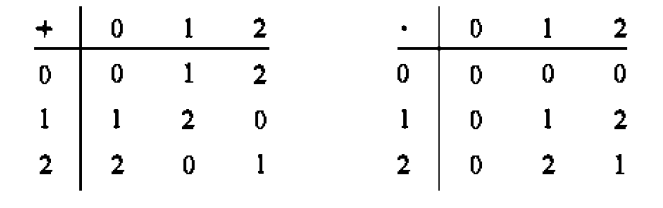
\includegraphics[scale=0.7]{classarithmetic.png}
    \caption{New notation for $\mathbb{Z}_3$}\label{fig:New notation for Z sub 3}
\end{figure}

\subsection*{The structure of $\mathbb{Z}_p$ when $p$ is Prime}

Not all $\Z_n$ share the same properties of $\Z$, in $\Z$ the product of and nonzero integer is nonzero, however
in $\Z_6$ we have $2 \cdot 3 = 0$. On the other hand in $\Z_5$ we have that the product of nonzero elements is always
nonzero. $\Z_5$ has, for any $a\neq0$, the equation $ax=1$ has a solution in $\Z_5$.

\subsection*{Theorem 2.8}
If $p > 1$ is an integer, the following conditions are equivalent:
\begin{enumerate}
    \item p is prime
    \item For any $a\neq0$, the equation $ax=1$ has a solution in $\Z_p$.
    \item Whenever $bc=0$ in $\Z_p$, at least one of $b$ and $c$ is zero.
\end{enumerate}
\subsection*{Example:}
In $\Z_3$ if $a = 2$ then $ax=1$ has a solution in $\Z_3$ of $2$. And $0 \cdot 1 = 0$ and $0 \cdot 2 = 0$ and $1 \cdot 2 = 2$.

\subsection*{The structure of $\mathbb{Z}_n$}
When $n$ is not prime, the equation doesn't have to have a solution to $ax=1$. For an example, the equation $2x=1$ has no solution
in $\Z_4$

\subsection*{Theorem 2.9}
Let $a$ and $n$ be integers with $n > 1$. Then
\begin{center}
    The equation $[a]x=[1]$ has a solution in $\Z_n$ if and only if $(a,n)=1$ in $\Z$.
\end{center}
\subsection*{Units and Zero Divisors}
An element $a$ in $\Z_n$ is a unit if $[a]x=[1]$ has a solution in $\Z_n$. In other words $a$ is a unit if
there is another element $b$ in $\Z_n$ such that $ab=1$. In this case we say that $b$ is the inverse of $a$.
\subsection*{Theorem 2.10}
Let $a$ and $n$ be integers with $n > 1$. Then
\begin{center}
    $[a]$ is a unit of $\Z_n$ if and only if $(a,n)=1$ in $\Z$.
\end{center}

A nonzero element $a$ in $\Z_n$ is a zero divisor if $[a]x=[0]$ has a \textit{nonzero} solution in 
$\Z_n$(That is, if there is a nonzero element $c$ in $\Z_n$ such that $ac=0$).
\end{document}